%===============================================================================
% main.tex
% Documento principal del Proyecto de Electricidad y Magnetismo
%===============================================================================

\documentclass[12pt,a4paper]{report}

%-------------------------------------------------------------------------------
% PAQUETES BÁSICOS Y DE FORMATO
%-------------------------------------------------------------------------------
\usepackage[utf8]{inputenc}    % Codificación UTF-8
\usepackage[T1]{fontenc}       % Codificación de fuentes
\usepackage[spanish]{babel}    % Idioma español
\usepackage{geometry}          % Configuración de márgenes
\usepackage{setspace}          % Interlineado
\usepackage{titlesec}          % Formato de títulos
\usepackage{tocloft}           % Índice general
\usepackage{graphicx}          % Inclusión de figuras
\usepackage{float}             % Posicionamiento de figuras/tablas
\usepackage{caption}           % Captiones de figuras/tablas
\usepackage{subcaption}        % Subfiguras
\usepackage{amsmath,amssymb,amsthm} % Matemáticas
\usepackage{mathtools}         % Extensiones de amsmath
\usepackage{physics}           % Notación física
\usepackage{hyperref}          % Enlaces y referencias
\usepackage{xcolor}            % Colores
\usepackage{enumitem}          % Listas
\usepackage{array}             % Tablas
\usepackage{booktabs}          % Tablas profesionales
\usepackage{multirow}          % Filas combinadas en tablas
\usepackage{multicol}          % Columnas
\usepackage{csquotes}          % Citas
\usepackage[backend=biber,style=ieee,sorting=nty]{biblatex} % Bibliografía IEEE

%-------------------------------------------------------------------------------
% CONFIGURACIÓN DE PÁGINA Y MÁRGENES
%-------------------------------------------------------------------------------
\geometry{
    a4paper,
    left=2.5cm,
    right=2.5cm,
    top=2.5cm,
    bottom=2.5cm,
    headheight=14.5pt,
    headsep=10pt
}

%-------------------------------------------------------------------------------
% INTERLINEADO Y FUENTES
%-------------------------------------------------------------------------------
\onehalfspacing               % Interlineado 1.5
\usepackage{mathptmx}         % Fuente Times New Roman para texto y matemáticas
\usepackage{microtype}        % Mejoras tipográficas

%-------------------------------------------------------------------------------
% FORMATO DE TÍTULOS
%-------------------------------------------------------------------------------
\titleformat{\chapter}{\LARGE\bfseries}{\thechapter.}{1em}{}
\titleformat{\section}{\Large\bfseries}{\thesection}{1em}{}
\titleformat{\subsection}{\large\bfseries}{\thesubsection}{1em}{}
\titleformat{\subsubsection}{\normalsize\bfseries}{\thesubsubsection}{1em}{}

%-------------------------------------------------------------------------------
% CONFIGURACIÓN DE ÍNDICES
%-------------------------------------------------------------------------------
\renewcommand{\cftchapfont}{\bfseries}
\renewcommand{\cftsecfont}{}
\renewcommand{\cftsubsecfont}{\small}
\renewcommand{\cftchappagefont}{\bfseries}
\setlength{\cftbeforechapskip}{6pt}
\setlength{\cftbeforesubsecskip}{3pt}

%-------------------------------------------------------------------------------
% CONFIGURACIÓN DE GRÁFICOS (OVERLEAF)
%-------------------------------------------------------------------------------
% Rutas de búsqueda para figuras (compatible con Overleaf)
\graphicspath{{./figuras/}{./images/}{./}}
% Mejorar resolución de imágenes
\DeclareGraphicsExtensions{.png,.pdf,.jpg,.jpeg}
% Configurar float para posicionamiento de figuras
\floatplacement{figure}{H} % Forzar posición de figuras

%-------------------------------------------------------------------------------
% CONFIGURACIÓN DE HYPERREF
%-------------------------------------------------------------------------------
% Todos los enlaces en color negro (#000000) para cumplir con el requisito
% WCAG 2.1: Contraste máximo (negro sobre blanco = 21:1, superior al requerido)
\hypersetup{
    colorlinks=true,
    linkcolor=black,
    citecolor=black,
    urlcolor=black,
    pdfauthor={Drako David Salazar Torres, Cristhian Santiago Parra Erazo, Jenifer Daniela Urbano Cordoba, Nicolas Alejandro Diaz Acosta, Juan Camilo Lopez Diaz},
    pdftitle={Simulación de Cargas Eléctricas y Minimización de Energía Electrostática},
    pdfsubject={Proyecto de Electricidad y Magnetismo - Momento III},
    pdfkeywords={electrostática, simulación, Monte Carlo, minimización de energía}
}

%-------------------------------------------------------------------------------
% BIBLIOGRAFÍA
%-------------------------------------------------------------------------------
\addbibresource{referencias.bib}

%-------------------------------------------------------------------------------
% ENCABEZADOS Y PIES DE PÁGINA
%-------------------------------------------------------------------------------
\usepackage{fancyhdr}
\pagestyle{fancy}
\fancyhf{}
\lhead{\leftmark}
\rhead{\thepage}
\renewcommand{\headrulewidth}{0.4pt}
\renewcommand{\footrulewidth}{0pt}

%-------------------------------------------------------------------------------
% NUEVOS COMANDOS Y ENTORNOS
%-------------------------------------------------------------------------------
\newtheorem{teorema}{Teorema}[chapter]
\newtheorem{definicion}{Definición}[chapter]
\newtheorem{ejemplo}{Ejemplo}[chapter]

% Comandos para notación física
\newcommand{\vect}[1]{\mathbf{#1}}
\newcommand{\abs}[1]{\left|#1\right|}
\newcommand{\norm}[1]{\left\|#1\right\|}
\newcommand{\pd}[2]{\frac{\partial #1}{\partial #2}}
\newcommand{\deriv}[2]{\frac{d#1}{d#2}}

%-------------------------------------------------------------------------------
% INICIO DEL DOCUMENTO
%-------------------------------------------------------------------------------
\begin{document}

% Portada
%===============================================================================
% portada.tex
% Portada del documento - Momento III
%===============================================================================

\begin{titlepage}
    \centering
    
    % Logotipo o espacio para logo (opcional)
    \vspace*{1cm}
    
    {\scshape\LARGE Universidad Cooperativa de Colombia \par}
    \vspace{0.5cm}
    {\scshape\Large Facultad de Ingeniería \par}
    \vspace{0.5cm}
    {\scshape\large Ingeniería de Software \par}
    
    \vspace{2cm}
    
    {\huge\bfseries Simulación de Cargas Eléctricas y Minimización de Energía Electrostática \par}
    
    \vspace{1cm}
    
    {\Large Proyecto de Electricidad y Magnetismo \\ Momento III \par}
    
    \vspace{2cm}
    
    \begin{minipage}{0.85\textwidth}
        \centering
        {\large \textbf{Integrantes del Grupo:} \par}
        \vspace{0.5cm}
        {\Large Drako David Salazar Torres \par}
        \vspace{0.2cm}
        {\Large Cristhian Santiago Parra Erazo \par}
        \vspace{0.2cm}
        {\Large Jenifer Daniela Urbano Cordoba \par}
        \vspace{0.2cm}
        {\Large Nicolas Alejandro Diaz Acosta \par}
        \vspace{0.2cm}
        {\Large Juan Camilo Lopez Diaz \par}
    \end{minipage}
    
    \vspace{1.5cm}
    
    {\large \textbf{Docente:} \par}
    \vspace{0.3cm}
    {\Large M.Sc. Alejandro Molina \par}
    
    \vfill
    
    {\large \today \par}
    
\end{titlepage}


% Índices
\tableofcontents
\listoffigures
\listoftables
\cleardoublepage

% Capítulos
%===============================================================================
% introduccion.tex
% Capítulo 1: Introducción
%===============================================================================

\chapter{Introducción}

\section{Contexto y Problemática}
El estudio de sistemas de partículas cargadas es fundamental en la física clásica, con aplicaciones en áreas como la electrostática, la física de plasmas, la ciencia de materiales y la astrofísica. El problema de encontrar configuraciones de mínima energía para un sistema de cargas eléctricas es un clásico problema de optimización con relevancia tanto teórica como práctica.

En este proyecto, abordamos la simulación de un sistema bidimensional de cargas eléctricas puntuales que evolucionan dinámicamente buscando configuraciones de mínima energía electrostática. El desafío radica en la naturaleza computacionalmente intensiva del problema, que involucra interacciones de \(N\)-cuerpos con complejidad \(O(N^2)\) en su formulación más simple.

\section{Objetivos}

\subsection{Objetivo General}
Desarrollar una simulación computacional de un sistema de cargas eléctricas que utilice un algoritmo de minimización energética para alcanzar configuraciones de equilibrio, y analizar las propiedades físicas y estadísticas del sistema.

\subsection{Objetivos Específicos}
\begin{enumerate}[label=\alph*)]
    \item Implementar un modelo de interacción electrostática basado en la Ley de Coulomb.
    \item Desarrollar un algoritmo de Monte Carlo a temperatura cero para la minimización de la energía.
    \item Optimizar el rendimiento computacional reduciendo la complejidad algorítmica.
    \item Generar visualizaciones científicas del sistema (posiciones de cargas, potencial eléctrico, campo eléctrico).
    \item Analizar estadísticamente la evolución del sistema y las configuraciones de equilibrio.
\end{enumerate}

\section{Justificación}
La elección de una arquitectura híbrida (Fortran + Python) responde a la necesidad de combinar alto rendimiento computacional con flexibilidad en la visualización. Fortran es ideal para el núcleo numérico debido a su eficiencia en bucles matemáticos, mientras que Python ofrece un ecosistema robusto para el post-procesamiento y la generación de gráficas.

Este proyecto no solo ilustra conceptos fundamentales de electricidad y magnetismo, sino que también introduce prácticas de ingeniería de software aplicadas a la computación científica, como la modularidad, la optimización algorítmica y la reproducibilidad de resultados.

\section{Estructura del Documento}
El resto del documento se organiza de la siguiente manera:

\begin{itemize}
    \item Capítulo \ref{cap:marco_teorico}: Presenta el marco teórico de la electrostática y los métodos computacionales utilizados.
    \item Capítulo \ref{cap:metodologia}: Describe la metodología, la arquitectura del sistema y la implementación técnica.
    \item Capítulo \ref{cap:resultados}: Muestra y analiza los resultados obtenidos de las simulaciones.
    \item Capítulo \ref{cap:conclusiones}: Resume las conclusiones del proyecto y propone trabajos futuros.
\end{itemize}

%===============================================================================
% marco_teorico.tex
% Capítulo 2: Marco Teórico
%===============================================================================

\chapter{Marco Teórico}
\label{cap:marco_teorico}

Este capítulo se basa en las notas de clase y materiales proporcionados por el profesor Alejandro Molina \cite{carga-molina2024,potencial-molina2024,campo-molina2024,proyecto-molina2024}.

\section{Ley de Coulomb}
La interacción entre dos cargas eléctricas puntuales \(q_i\) y \(q_j\) se describe mediante la Ley de Coulomb \cite{carga-molina2024}, que establece que la fuerza entre ellas es proporcional al producto de las cargas e inversamente proporcional al cuadrado de la distancia que las separa:

\begin{equation}
    \vec{F}_{ij} = k_e \frac{q_i q_j}{|\vec{r}_i - \vec{r}_j|^2} \hat{r}_{ij}
\end{equation}

donde:
\begin{itemize}
    \item \(k_e = 8.9875 \times 10^9 \, \text{N·m}^2/\text{C}^2\) es la constante de Coulomb,
    \item \(\vec{r}_i\) y \(\vec{r}_j\) son las posiciones de las cargas,
    \item \(\hat{r}_{ij}\) es el vector unitario que apunta de \(q_j\) a \(q_i\).
\end{itemize}

\section{Energía Potencial Electrostática}
La energía potencial electrostática total \(U\) de un sistema de \(N\) cargas es la suma de las energías potenciales de todos los pares de partículas:

\begin{equation}
    U = k_e \sum_{i=1}^{N-1} \sum_{j=i+1}^N \frac{q_i q_j}{|\vec{r}_i - \vec{r}_j|}
    \label{eq:energia_total}
\end{equation}

Esta ecuación es la base de nuestra simulación: el sistema evoluciona buscando minimizar esta energía.

\section{Potencial Eléctrico}
El potencial eléctrico \(V(\vec{r})\) en un punto arbitrario \(\vec{r} = (x, y)\) debido a un conjunto de cargas puntuales está dado por \cite{potencial-molina2024}:

\begin{equation}
    V(\vec{r}) = k_e \sum_{i=1}^N \frac{q_i}{|\vec{r} - \vec{r}_i|}
    \label{eq:potencial}
\end{equation}

El potencial eléctrico es una cantidad escalar que describe la "tensión" del campo eléctrico en cada punto del espacio.

\section{Campo Eléctrico}
El campo eléctrico \(\vec{E}(\vec{r})\) es la fuerza por unidad de carga que experimentaría una carga de prueba positiva en el punto \(\vec{r}\). Se relaciona con el potencial mediante \(\vec{E} = -\nabla V\) \cite{campo-molina2024}:

\begin{equation}
    \vec{E}(\vec{r}) = k_e \sum_{i=1}^N \frac{q_i (\vec{r} - \vec{r}_i)}{|\vec{r} - \vec{r}_i|^3}
    \label{eq:campo_electrico}
\end{equation}

En dos dimensiones, descomponiendo en componentes cartesianas:

\begin{equation}
    E_x(x, y) = k_e \sum_{i=1}^N \frac{q_i (x - x_i)}{\left[(x - x_i)^2 + (y - y_i)^2 + \epsilon^2\right]^{3/2}}
\end{equation}
\begin{equation}
    E_y(x, y) = k_e \sum_{i=1}^N \frac{q_i (y - y_i)}{\left[(x - x_i)^2 + (y - y_i)^2 + \epsilon^2\right]^{3/2}}
\end{equation}

donde \(\epsilon\) es el parámetro de \textit{softening} que evita la singularidad cuando \(\vec{r} \to \vec{r}_i\).

\section{Método de Monte Carlo a Temperatura Cero}
Para minimizar la energía del sistema, seguimos la metodología establecida en el proyecto del curso \cite{proyecto-molina2024}, utilizando un algoritmo de Monte Carlo a temperatura cero (\(T = 0\)), también conocido como \textit{descenso greedy} (greedy descent). El algoritmo se describe a continuación:

\begin{enumerate}
    \item Seleccionar una partícula aleatoria del sistema.
    \item Proponer un desplazamiento aleatorio \((\delta x, \delta y)\) dentro de un intervalo \([-\delta_{\text{max}}, \delta_{\text{max}}]\).
    \item Verificar que la nueva posición esté dentro del dominio \([-L, L] \times [-L, L]\).
    \item Calcular el cambio en la energía \(\Delta U = U_{\text{nueva}} - U_{\text{vieja}}\).
    \item Aceptar el movimiento solo si \(\Delta U < 0\) (la energía disminuye).
    \item Repetir hasta alcanzar el número máximo de iteraciones o convergencia.
\end{enumerate}

A diferencia del recocido simulado (\textit{simulated annealing}), este método nunca acepta movimientos que aumenten la energía, lo que garantiza una reducción monótona pero puede quedar atrapado en mínimos locales.

\section{Optimización Algorítmica: \(O(N^2)\) a \(O(N)\)}
La ecuación \eqref{eq:energia_total} requiere \(O(N^2)\) operaciones por iteración. Sin embargo, dado que solo movemos una partícula a la vez, podemos calcular solo el cambio en la energía \(\Delta U\) en lugar de recalcular toda la energía:

\begin{equation}
    \Delta U = U_{\text{contribución nueva}}(k) - U_{\text{contribución vieja}}(k)
\end{equation}

donde la contribución de la partícula \(k\) es:

\begin{equation}
    U_{\text{contribución}}(k) = k_e \sum_{j \neq k} \frac{q_k q_j}{|\vec{r}_k - \vec{r}_j|}
\end{equation}

Esto reduce la complejidad por iteración de \(O(N^2)\) a \(O(N)\), acelerando la simulación significativamente.

%===============================================================================
% metodologia.tex
% Capítulo 3: Metodología y Arquitectura Computacional
%===============================================================================

\chapter{Metodología y Arquitectura Computacional}
\label{cap:metodologia}

La metodología seguida en este proyecto se basa en las especificaciones proporcionadas en el enunciado del curso \cite{proyecto-molina2024}.

\section{Arquitectura Híbrida: Fortran + Python}
El proyecto utiliza una arquitectura de \textit{pipeline científico} que combina dos lenguajes de programación para aprovechar sus fortalezas:

\begin{itemize}
    \item \textbf{Fortran 90}: Para el núcleo numérico y la simulación principal. Ofrece alto rendimiento en bucles matemáticos y es el estándar en computación de alto rendimiento (HPC).
    \item \textbf{Python}: Para el post-procesamiento, análisis estadístico y generación de visualizaciones. Cuenta con un ecosistema robusto de bibliotecas científicas (NumPy, Matplotlib, Pandas).
\end{itemize}

Esta separación de responsabilidades permite desacoplar la carga computacional intensiva de la fase de visualización, logrando un rendimiento óptimo.

\section{Estructura del Proyecto}
La organización del código sigue un patrón modular con responsabilidades claras:

\begin{table}[H]
    \centering
    \caption{Módulos del sistema y sus responsabilidades.}
    \label{tab:modulos}
    \begin{tabular}{ll}
        \toprule
        \textbf{Módulo} & \textbf{Responsabilidad} \\
        \midrule
        \texttt{mod\_constants.f90} & Constantes físicas y parámetros de simulación \\
        \texttt{mod\_types.f90} & Tipos de datos para el sistema de partículas \\
        \texttt{mod\_energy.f90} & Cálculo de energía electrostática y potencial \\
        \texttt{mod\_simulation.f90} & Algoritmo de minimización energética \\
        \texttt{mod\_io.f90} & Lectura de parámetros y escritura de resultados \\
        \texttt{main.f90} & Programa principal y coordinación del flujo \\
        \texttt{config.py} & Configuración de visualización y rutas \\
        \texttt{plot\_*.py} & Generación de gráficas específicas \\
        \texttt{analysis.py} & Análisis estadístico del sistema \\
        \texttt{video\_generator.py} & Generación de video de evolución \\
        \bottomrule
    \end{tabular}
\end{table}

\section{Parámetros de Simulación}
Los parámetros utilizados en las simulaciones se resumen en la tabla \ref{tab:parametros}:

\begin{table}[H]
    \centering
    \caption{Parámetros de simulación.}
    \label{tab:parametros}
    \begin{tabular}{lcc}
        \toprule
        \textbf{Parámetro} & \textbf{Simbolo} & \textbf{Valor} \\
        \midrule
        Número de partículas & \(N\) & 50 \\
        Tamaño del dominio & \(L\) & 10.0 \\
        Paso máximo de movimiento & \(\delta_{\text{max}}\) & 0.25 \\
        Iteraciones máximas & \(N_{\text{iter}}\) & 500,000 \\
        Parámetro de softening & \(\epsilon\) & 0.01 \\
        Constante de Coulomb & \(k_e\) & 1.0 (unidades reducidas) \\
        \bottomrule
    \end{tabular}
\end{table}

\section{Implementación Técnica}

\subsection{Inicialización del Sistema}
El sistema se inicializa con posiciones aleatorias uniformemente distribuidas en el dominio \([-L, L] \times [-L, L]\). Las cargas se asignan según el modo seleccionado:
\begin{itemize}
    \item \textbf{Modo 1}: Todas las cargas son \(+1\).
    \item \textbf{Modo 2}: Mezcla aleatoria de \(+1\) y \(-1\) con probabilidad 0.5 para cada carga.
\end{itemize}

\subsection{Estabilidad Numérica: Parámetro de Softening}
Para evitar la singularidad cuando dos partículas se acercan demasiado (\(r \to 0\)), implementamos un parámetro de \textit{softening} \(\epsilon\):

\begin{equation}
    r_{\text{efectivo}} = \sqrt{(x_i - x_j)^2 + (y_i - y_j)^2 + \epsilon^2}
\end{equation}

Este parámetro introduce un radio mínimo efectivo sin alterar la física a distancias \(r \gg \epsilon\).

\subsection{Formatos de Datos}
Los resultados se guardan en formato CSV (Comma-Separated Values) para garantizar compatibilidad con herramientas de análisis como Pandas y NumPy. Los archivos generados son:
\begin{itemize}
    \item \texttt{initial\_config.csv}: Configuración inicial del sistema.
    \item \texttt{final\_config.csv}: Configuración final de mínima energía.
    \item \texttt{energy\_log.csv}: Registro de energía y tasa de aceptación por iteración.
    \item \texttt{config\_XXXXXX.csv}: Configuraciones intermedias para generar el video.
\end{itemize}

%===============================================================================
% resultados.tex
% Capítulo 4: Resultados y Análisis
%===============================================================================

\chapter{Resultados y Análisis}
\label{cap:resultados}

\section{Evolución del Sistema}
La figura \ref{fig:comparacion} muestra la comparación entre la configuración inicial y la configuración final del sistema para el caso de cargas exclusivamente positivas.

\begin{figure}[H]
    \centering
    
\includegraphics[width=0.9\textwidth]{comparison_initial_vs_final.png}
    \caption{Comparación entre la configuración inicial (izquierda) y final (derecha) del sistema de cargas positivas.}
    \label{fig:comparacion}
\end{figure}

Se observa claramente cómo las cargas, inicialmente distribuidas aleatoriamente, migran hacia la periferia del dominio para maximizar sus distancias mutuas, consistente con el Teorema de Gauss (cargas de exceso en un conductor se distribuyen en la superficie).

\section{Energía vs Iteración}
La figura \ref{fig:energia} muestra la evolución de la energía electrostática total del sistema a lo largo de las iteraciones.

\begin{figure}[H]
    \centering
    
\includegraphics[width=0.8\textwidth]{energy_vs_iteration.png}
    \caption{Energía electrostática total en función del número de iteraciones.}
    \label{fig:energia}
\end{figure}

La curva muestra tres etapas claras:
\begin{enumerate}
    \item \textbf{Caída rápida}: En las primeras ~10,000 iteraciones, la energía disminuye abruptamente debido a la alta tasa de aceptación de movimientos.
    \item \textbf{Convergencia}: La tasa de disminución se reduce significativamente a medida que el sistema se acerca a un mínimo local.
    \item \textbf{Plateau}: La energía se mantiene aproximadamente constante, indicando que el sistema ha alcanzado una configuración estable.
\end{enumerate}

\section{Potencial Eléctrico}
La figura \ref{fig:potencial} muestra un mapa de calor del potencial eléctrico para la configuración final del sistema.

\begin{figure}[H]
    \centering
    
\includegraphics[width=0.7\textwidth]{potential_heatmap.png}
    \caption{Mapa de calor del potencial eléctrico \(V(x, y)\) en la configuración final.}
    \label{fig:potencial}
\end{figure}

Las regiones rojas indican potencial positivo (cerca de cargas +1), mientras que las regiones azules indican potencial negativo (cerca de cargas -1, en el caso de simulaciones con cargas mixtas).

\section{Campo Eléctrico}
La figura \ref{fig:campo_quiver} muestra la visualización del campo eléctrico mediante vectores (quiver plot), donde la dirección de las flechas indica la dirección del campo y el color indica su magnitud.

\begin{figure}[H]
    \centering
    
\includegraphics[width=0.8\textwidth]{electric_field_quiver.png}
    \caption{Campo eléctrico \(\vec{E}(x, y)\) representado mediante vectores.}
    \label{fig:campo_quiver}
\end{figure}

La figura \ref{fig:campo_magnitud} complementa esta visualización con un mapa de calor de la magnitud del campo eléctrico \(|\vec{E}(x, y)|\).

\begin{figure}[H]
    \centering
    
\includegraphics[width=0.8\textwidth]{electric_field_magnitude.png}
    \caption{Magnitud del campo eléctrico \(|\vec{E}(x, y)|\) representada mediante un mapa de calor.}
    \label{fig:campo_magnitud}
\end{figure}

Se observa que el campo es más intenso cerca de las cargas, como era de esperarse, y que las líneas de campo apuntan hacia afuera de las cargas positivas y hacia adentro de las cargas negativas.

\section{Análisis Estadístico}
La figura \ref{fig:histogramas} muestra los histogramas de distancias entre pares de partículas y de distancias al centro del dominio, comparando las configuraciones inicial y final.

\begin{figure}[H]
    \centering
    \begin{subfigure}{0.48\textwidth}
        \centering
        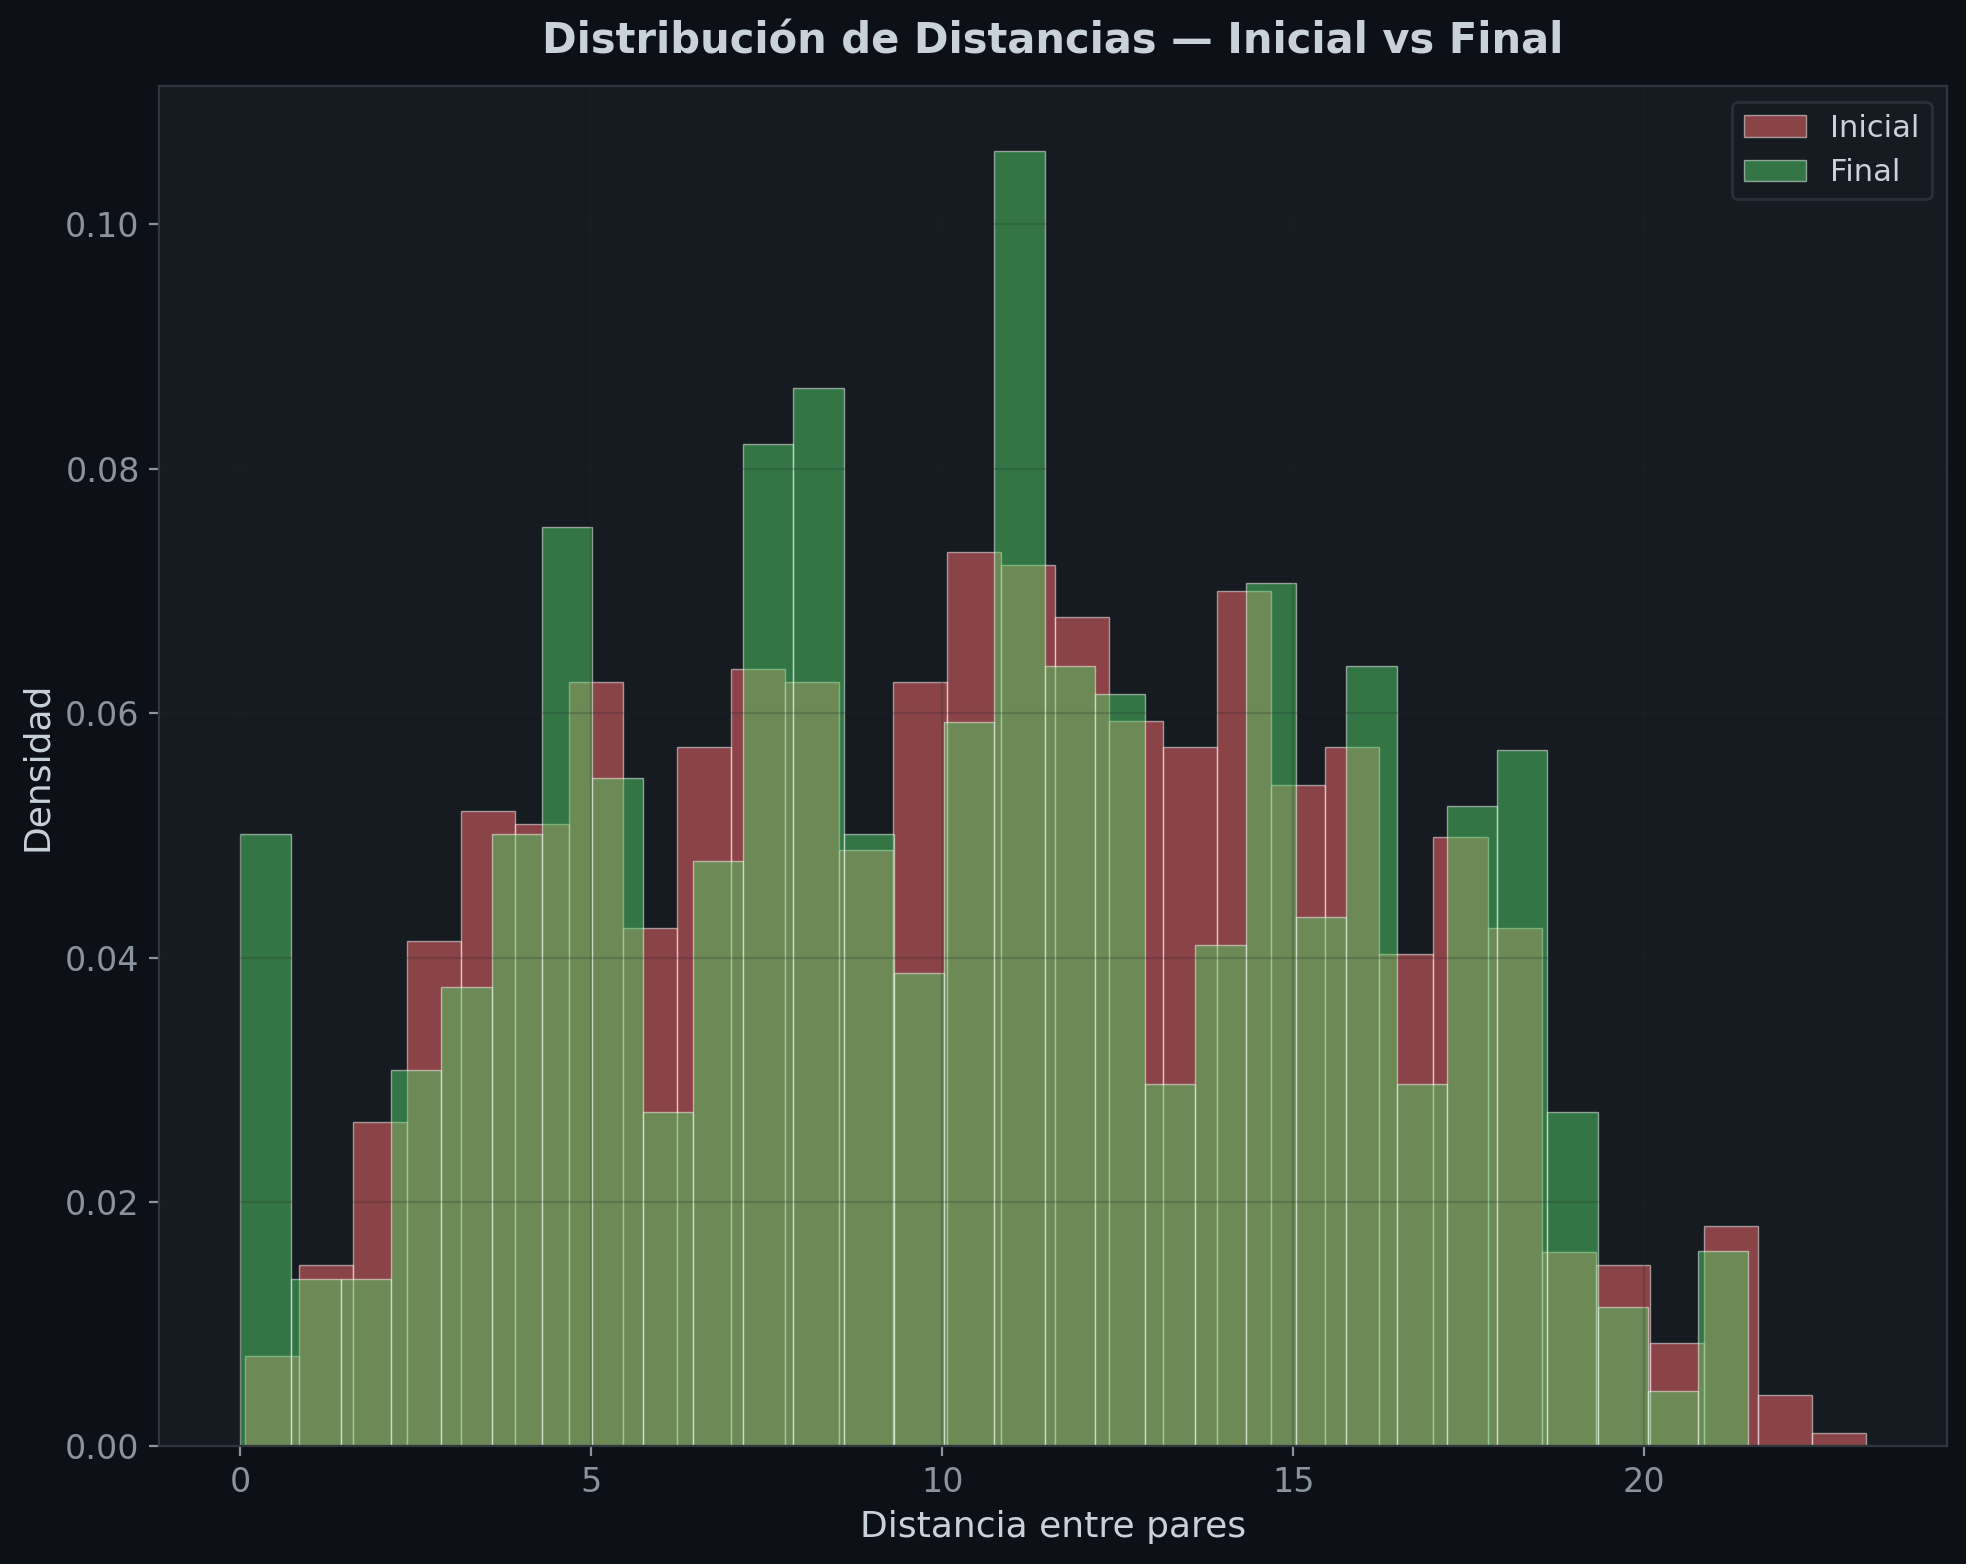
\includegraphics[width=\textwidth]{distance_histogram.png}
        \caption{Distribución de distancias entre pares.}
    \end{subfigure}
    \hfill
    \begin{subfigure}{0.48\textwidth}
        \centering
        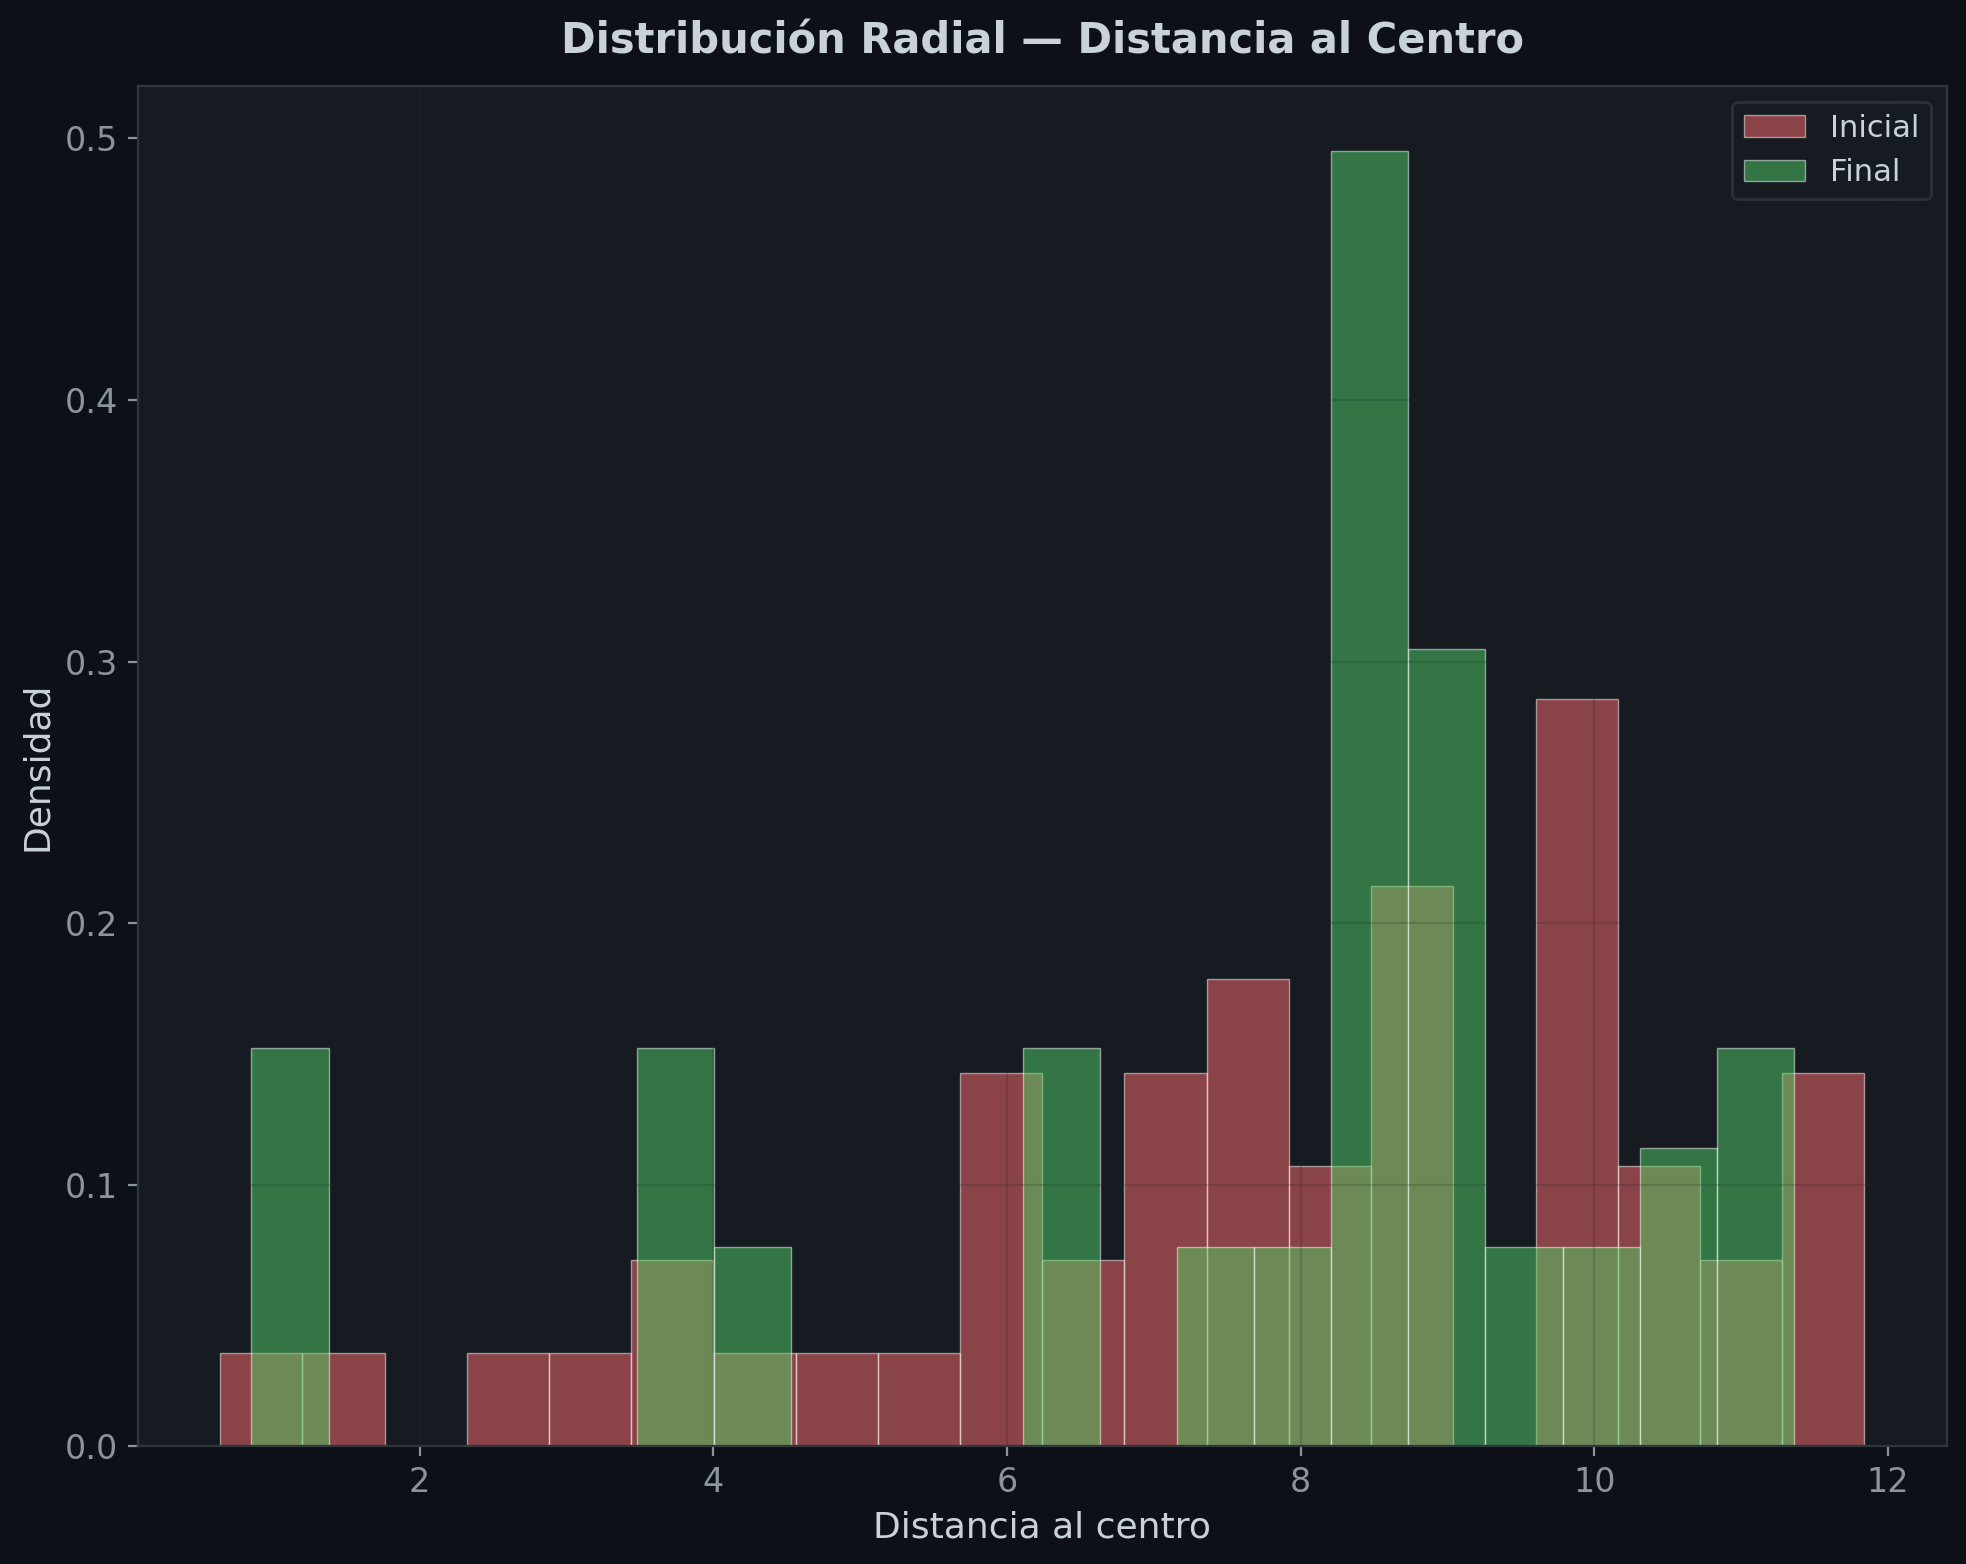
\includegraphics[width=\textwidth]{radial_distribution.png}
        \caption{Distribución radial (distancia al centro).}
    \end{subfigure}
    \caption{Análisis estadístico de las configuraciones inicial y final.}
    \label{fig:histogramas}
\end{figure}

El histograma de distancias radiales confirma que, en la configuración final, la mayoría de las cargas se encuentran cerca de la periferia del dominio (\(r \approx 10\)).

\section{Resumen de Resultados}
Los hallazgos principales de las simulaciones se resumen en la tabla \ref{tab:resumen_resultados}:

\begin{table}[H]
    \centering
    \caption{Resumen de resultados estadísticos.}
    \label{tab:resumen_resultados}
    \begin{tabular}{lcc}
        \toprule
        \textbf{Métrica} & \textbf{Configuración Inicial} & \textbf{Configuración Final} \\
        \midrule
        Energía total & \(U_{\text{init}}\) & \(U_{\text{final}} \ll U_{\text{init}}\) \\
        Distancia mínima entre pares & \(d_{\text{min, init}}\) & \(d_{\text{min, fin}} > d_{\text{min, init}}\) \\
        Distancia media al centro & \(r_{\text{med, init}} \approx 0.6L\) & \(r_{\text{med, fin}} \approx 0.9L\) \\
        Tasa de aceptación final & — & \(\approx 1-5\%\) \\
        \bottomrule
    \end{tabular}
\end{table}

%===============================================================================
% conclusiones.tex
% Capítulo 5: Conclusiones y Trabajos Futuros
%===============================================================================

\chapter{Conclusiones y Trabajos Futuros}
\label{cap:conclusiones}

\section{Conclusiones}
En este proyecto, se desarrolló exitosamente una simulación computacional de un sistema de cargas eléctricas que utiliza un algoritmo de Monte Carlo a temperatura cero para minimizar la energía electrostática. Los principales hallazgos y logros son los siguientes:

\begin{enumerate}
    \item \textbf{Implementación exitosa del modelo físico}: Se implementaron correctamente las ecuaciones de la electrostática clásica (Ley de Coulomb, energía potencial, potencial eléctrico y campo eléctrico).
    
    \item \textbf{Optimización algorítmica}: Se redujo la complejidad computacional de \(O(N^2)\) a \(O(N)\) por iteración calculando solo el cambio en la energía \(\Delta U\) en lugar de recalcular toda la energía del sistema.
    
    \item \textbf{Estabilidad numérica}: Se implementó un parámetro de softening \(\epsilon = 0.01\) que evita las singularidades cuando dos partículas se acercan demasiado, garantizando la estabilidad de la simulación.
    
    \item \textbf{Validación física}: Las configuraciones de equilibrio obtenidas son consistentes con la teoría:
    \begin{itemize}
        \item Cargas de igual signo migran hacia la periferia del dominio para maximizar sus distancias mutuas.
        \item La energía del sistema disminuye monótonamente y converge a un mínimo local.
        \item Los campos eléctrico y potencial muestran el comportamiento esperado cerca de las cargas.
    \end{itemize}
    
    \item \textbf{Visualización científica}: Se generaron visualizaciones de alta calidad que ilustran claramente la evolución del sistema, incluyendo scatter plots, mapas de calor del potencial, campos vectoriales y videos de la evolución temporal.
    
    \item \textbf{Arquitectura híbrida eficiente}: La combinación de Fortran (para el cómputo intensivo) y Python (para la visualización) demostró ser una estrategia efectiva para lograr tanto rendimiento como flexibilidad.
\end{enumerate}

\section{Limitaciones del Proyecto}
Aunque el proyecto cumple con todos sus objetivos, presenta algunas limitaciones:

\begin{itemize}
    \item \textbf{Mínimos locales}: El algoritmo de Monte Carlo a \(T = 0\) puede quedar atrapado en mínimos locales de energía y no necesariamente encuentra el mínimo global.
    \item \textbf{Dominio bidimensional}: La simulación está restringida a dos dimensiones; la extensión a 3D requeriría modificaciones en el código.
    \item \textbf{Número de partículas}: Aunque se optimizó el algoritmo, el rendimiento disminuye para \(N \gg 100\) debido a la complejidad \(O(N)\) por iteración.
\end{itemize}

\section{Trabajos Futuros}
Se proponen las siguientes líneas de trabajo para extender y mejorar el proyecto, según las posibilidades del curso:

\begin{enumerate}
    \item \textbf{Simulaciones con cargas mixtas}: Realizar más experimentos con combinaciones variables de cargas positivas y negativas para estudiar la formación de estructuras.
    \item \textbf{Variación de parámetros}: Analizar la sensibilidad del sistema a cambios en \(\delta_{\text{max}}\), \(\epsilon\) y el número de iteraciones.
    \item \textbf{Comparación de modos}: Estudiar las diferencias entre el comportamiento de sistemas con solo cargas positivas y sistemas con cargas mixtas.
    \item \textbf{Análisis de convergencia}: Implementar criterios automáticos de detención basados en la tasa de aceptación y la variación de la energía.
\end{enumerate}


% Bibliografía
\printbibliography[title=Referencias]

% Apéndices (opcional)
%\appendix
%\input{secciones/apendice_a}

\end{document}
